% Options for packages loaded elsewhere
\PassOptionsToPackage{unicode}{hyperref}
\PassOptionsToPackage{hyphens}{url}
%
\documentclass[
]{article}
\usepackage{amsmath,amssymb}
\usepackage{lmodern}
\usepackage{iftex}
\ifPDFTeX
  \usepackage[T1]{fontenc}
  \usepackage[utf8]{inputenc}
  \usepackage{textcomp} % provide euro and other symbols
\else % if luatex or xetex
  \usepackage{unicode-math}
  \defaultfontfeatures{Scale=MatchLowercase}
  \defaultfontfeatures[\rmfamily]{Ligatures=TeX,Scale=1}
\fi
% Use upquote if available, for straight quotes in verbatim environments
\IfFileExists{upquote.sty}{\usepackage{upquote}}{}
\IfFileExists{microtype.sty}{% use microtype if available
  \usepackage[]{microtype}
  \UseMicrotypeSet[protrusion]{basicmath} % disable protrusion for tt fonts
}{}
\makeatletter
\@ifundefined{KOMAClassName}{% if non-KOMA class
  \IfFileExists{parskip.sty}{%
    \usepackage{parskip}
  }{% else
    \setlength{\parindent}{0pt}
    \setlength{\parskip}{6pt plus 2pt minus 1pt}}
}{% if KOMA class
  \KOMAoptions{parskip=half}}
\makeatother
\usepackage{xcolor}
\IfFileExists{xurl.sty}{\usepackage{xurl}}{} % add URL line breaks if available
\IfFileExists{bookmark.sty}{\usepackage{bookmark}}{\usepackage{hyperref}}
\hypersetup{
  pdftitle={Milestone \#4},
  pdfauthor={Rachael Baartmans, Lara Petalio, Christine Truong},
  hidelinks,
  pdfcreator={LaTeX via pandoc}}
\urlstyle{same} % disable monospaced font for URLs
\usepackage[margin=1in]{geometry}
\usepackage{color}
\usepackage{fancyvrb}
\newcommand{\VerbBar}{|}
\newcommand{\VERB}{\Verb[commandchars=\\\{\}]}
\DefineVerbatimEnvironment{Highlighting}{Verbatim}{commandchars=\\\{\}}
% Add ',fontsize=\small' for more characters per line
\usepackage{framed}
\definecolor{shadecolor}{RGB}{248,248,248}
\newenvironment{Shaded}{\begin{snugshade}}{\end{snugshade}}
\newcommand{\AlertTok}[1]{\textcolor[rgb]{0.94,0.16,0.16}{#1}}
\newcommand{\AnnotationTok}[1]{\textcolor[rgb]{0.56,0.35,0.01}{\textbf{\textit{#1}}}}
\newcommand{\AttributeTok}[1]{\textcolor[rgb]{0.77,0.63,0.00}{#1}}
\newcommand{\BaseNTok}[1]{\textcolor[rgb]{0.00,0.00,0.81}{#1}}
\newcommand{\BuiltInTok}[1]{#1}
\newcommand{\CharTok}[1]{\textcolor[rgb]{0.31,0.60,0.02}{#1}}
\newcommand{\CommentTok}[1]{\textcolor[rgb]{0.56,0.35,0.01}{\textit{#1}}}
\newcommand{\CommentVarTok}[1]{\textcolor[rgb]{0.56,0.35,0.01}{\textbf{\textit{#1}}}}
\newcommand{\ConstantTok}[1]{\textcolor[rgb]{0.00,0.00,0.00}{#1}}
\newcommand{\ControlFlowTok}[1]{\textcolor[rgb]{0.13,0.29,0.53}{\textbf{#1}}}
\newcommand{\DataTypeTok}[1]{\textcolor[rgb]{0.13,0.29,0.53}{#1}}
\newcommand{\DecValTok}[1]{\textcolor[rgb]{0.00,0.00,0.81}{#1}}
\newcommand{\DocumentationTok}[1]{\textcolor[rgb]{0.56,0.35,0.01}{\textbf{\textit{#1}}}}
\newcommand{\ErrorTok}[1]{\textcolor[rgb]{0.64,0.00,0.00}{\textbf{#1}}}
\newcommand{\ExtensionTok}[1]{#1}
\newcommand{\FloatTok}[1]{\textcolor[rgb]{0.00,0.00,0.81}{#1}}
\newcommand{\FunctionTok}[1]{\textcolor[rgb]{0.00,0.00,0.00}{#1}}
\newcommand{\ImportTok}[1]{#1}
\newcommand{\InformationTok}[1]{\textcolor[rgb]{0.56,0.35,0.01}{\textbf{\textit{#1}}}}
\newcommand{\KeywordTok}[1]{\textcolor[rgb]{0.13,0.29,0.53}{\textbf{#1}}}
\newcommand{\NormalTok}[1]{#1}
\newcommand{\OperatorTok}[1]{\textcolor[rgb]{0.81,0.36,0.00}{\textbf{#1}}}
\newcommand{\OtherTok}[1]{\textcolor[rgb]{0.56,0.35,0.01}{#1}}
\newcommand{\PreprocessorTok}[1]{\textcolor[rgb]{0.56,0.35,0.01}{\textit{#1}}}
\newcommand{\RegionMarkerTok}[1]{#1}
\newcommand{\SpecialCharTok}[1]{\textcolor[rgb]{0.00,0.00,0.00}{#1}}
\newcommand{\SpecialStringTok}[1]{\textcolor[rgb]{0.31,0.60,0.02}{#1}}
\newcommand{\StringTok}[1]{\textcolor[rgb]{0.31,0.60,0.02}{#1}}
\newcommand{\VariableTok}[1]{\textcolor[rgb]{0.00,0.00,0.00}{#1}}
\newcommand{\VerbatimStringTok}[1]{\textcolor[rgb]{0.31,0.60,0.02}{#1}}
\newcommand{\WarningTok}[1]{\textcolor[rgb]{0.56,0.35,0.01}{\textbf{\textit{#1}}}}
\usepackage{graphicx}
\makeatletter
\def\maxwidth{\ifdim\Gin@nat@width>\linewidth\linewidth\else\Gin@nat@width\fi}
\def\maxheight{\ifdim\Gin@nat@height>\textheight\textheight\else\Gin@nat@height\fi}
\makeatother
% Scale images if necessary, so that they will not overflow the page
% margins by default, and it is still possible to overwrite the defaults
% using explicit options in \includegraphics[width, height, ...]{}
\setkeys{Gin}{width=\maxwidth,height=\maxheight,keepaspectratio}
% Set default figure placement to htbp
\makeatletter
\def\fps@figure{htbp}
\makeatother
\setlength{\emergencystretch}{3em} % prevent overfull lines
\providecommand{\tightlist}{%
  \setlength{\itemsep}{0pt}\setlength{\parskip}{0pt}}
\setcounter{secnumdepth}{-\maxdimen} % remove section numbering
\usepackage{booktabs}
\usepackage{longtable}
\usepackage{array}
\usepackage{multirow}
\usepackage{wrapfig}
\usepackage{float}
\usepackage{colortbl}
\usepackage{pdflscape}
\usepackage{tabu}
\usepackage{threeparttable}
\usepackage{threeparttablex}
\usepackage[normalem]{ulem}
\usepackage{makecell}
\usepackage{xcolor}
\ifLuaTeX
  \usepackage{selnolig}  % disable illegal ligatures
\fi

\title{Milestone \#4}
\author{Rachael Baartmans, Lara Petalio, Christine Truong}
\date{11-14-22}

\begin{document}
\maketitle

\#\#Relevant Previous Importing and Data-cleaning Steps

\begin{verbatim}
## Warning in system("timedatectl", intern = TRUE): running command 'timedatectl'
## had status 1
\end{verbatim}

\begin{verbatim}
## -- Attaching packages --------------------------------------- tidyverse 1.3.1 --
\end{verbatim}

\begin{verbatim}
## v ggplot2 3.3.5     v purrr   0.3.4
## v tibble  3.1.6     v dplyr   1.0.8
## v tidyr   1.2.0     v stringr 1.4.0
## v readr   2.1.2     v forcats 0.5.1
\end{verbatim}

\begin{verbatim}
## -- Conflicts ------------------------------------------ tidyverse_conflicts() --
## x dplyr::filter() masks stats::filter()
## x dplyr::lag()    masks stats::lag()
\end{verbatim}

\begin{verbatim}
## 
## Attaching package: 'kableExtra'
\end{verbatim}

\begin{verbatim}
## The following object is masked from 'package:dplyr':
## 
##     group_rows
\end{verbatim}

\begin{verbatim}
## Rows: 1000 Columns: 24
## -- Column specification --------------------------------------------------------
## Delimiter: ","
## chr (24): ID, NERVOUS, WORRYING, PROBINTR, PROBDOWN, ASTHMA, HEARTDIS, DIABE...
## 
## i Use `spec()` to retrieve the full column specification for this data.
## i Specify the column types or set `show_col_types = FALSE` to quiet this message.
## Rows: 1000 Columns: 7
## -- Column specification --------------------------------------------------------
## Delimiter: ","
## chr (5): smokstat, HOWMANY, SMOK6UNI, BUYCALIF, WHEREBUY
## dbl (2): psraid, SMOK6NUM
## 
## i Use `spec()` to retrieve the full column specification for this data.
## i Specify the column types or set `show_col_types = FALSE` to quiet this message.
\end{verbatim}

\newpage

\hypertarget{milestone-4-assignments-delete-this-header-later}{%
\subsection{Milestone \#4 assignments (delete this header
later)}\label{milestone-4-assignments-delete-this-header-later}}

\hypertarget{calculating-pack-years}{%
\subsection{Calculating Pack-years}\label{calculating-pack-years}}

\begin{Shaded}
\begin{Highlighting}[]
\CommentTok{\#We calculated pack{-}years, which is given by the formula of}
\CommentTok{\#pack{-}years = \# of packs of cigarettes smoked per day * years a person has smoked.}
\CommentTok{\#This calculation led to the creation of a new variable called \textasciigrave{}pack\_years\textasciigrave{}.}
\CommentTok{\#\textasciigrave{}pack\_years\textasciigrave{} was created conditionally based on the three different time units}
\CommentTok{\#as determined by the existing variable \textasciigrave{}smok6uni\textasciigrave{}, which are: "Days", "Months",}
\CommentTok{\#and "Years". To change the unit of "Days" to years, we set up a conditional}
\CommentTok{\#statement in the code to divide \textasciigrave{}smok6num\textasciigrave{} by 365 before multiplying the result}
\CommentTok{\#by \textasciigrave{}packs\_per\_day\textasciigrave{} to get pack{-}years. Similarly, to change the unit of "Months"}
\CommentTok{\#to years, we set up a conditional statement in the code to divide \textasciigrave{}smok6num\textasciigrave{}}
\CommentTok{\#by 12 before multiplying the result by \textasciigrave{}packs\_per\_day\textasciigrave{} to get pack{-}years. For}
\CommentTok{\#\textasciigrave{}smok6uni\textasciigrave{} observations that have the value "Years", we just multiplied}
\CommentTok{\#\textasciigrave{}smok6num\textasciigrave{} by \textasciigrave{}packs\_per\_day\textasciigrave{} to get pack{-}years directly. We assigned}
\CommentTok{\#this overall change in the data frame smoker\_data\_2 to a new data frame}
\CommentTok{\#called smoker\_data\_3, which includes the new variable \textasciigrave{}pack\_years\textasciigrave{}.}

\NormalTok{smoker\_data\_3 }\OtherTok{\textless{}{-}}\NormalTok{ smoker\_data\_2 }\SpecialCharTok{\%\textgreater{}\%}
  \FunctionTok{mutate}\NormalTok{(}\AttributeTok{pack\_years =}
           \FunctionTok{case\_when}\NormalTok{(smok6uni }\SpecialCharTok{==} \StringTok{"Days"} \SpecialCharTok{\textasciitilde{}}\NormalTok{ packs\_per\_day}\SpecialCharTok{*}\NormalTok{(smok6num}\SpecialCharTok{/}\DecValTok{365}\NormalTok{),}
\NormalTok{                     smok6uni }\SpecialCharTok{==} \StringTok{"Months"} \SpecialCharTok{\textasciitilde{}}\NormalTok{ packs\_per\_day}\SpecialCharTok{*}\NormalTok{(smok6num}\SpecialCharTok{/}\DecValTok{12}\NormalTok{),}
\NormalTok{                     smok6uni }\SpecialCharTok{==} \StringTok{"Years"} \SpecialCharTok{\textasciitilde{}}\NormalTok{ packs\_per\_day}\SpecialCharTok{*}\NormalTok{(smok6num)))}

\CommentTok{\#We then rounded \textasciigrave{}pack\_years\textasciigrave{} to the nearest whole number for all observations.}

\NormalTok{smoker\_data\_3}\SpecialCharTok{$}\NormalTok{pack\_years }\OtherTok{\textless{}{-}} \FunctionTok{round}\NormalTok{(smoker\_data\_3}\SpecialCharTok{$}\NormalTok{pack\_years, }\DecValTok{0}\NormalTok{)}

\CommentTok{\#Afterwards, we viewed our new data frame, which includes our new variable}
\CommentTok{\#\textasciigrave{}pack\_years\textasciigrave{}.}

\NormalTok{smoker\_data\_3}
\end{Highlighting}
\end{Shaded}

\begin{verbatim}
## # A tibble: 1,000 x 9
##    psraid smokstat     wherebuy buycalif howmany smok6num smok6uni packs_per_day
##     <dbl> <chr>        <chr>    <chr>      <dbl>    <dbl> <chr>            <dbl>
##  1 100099 Current dai~ At othe~ In Cali~      30       36 Years             1.5 
##  2 100109 Current dai~ At toba~ In Cali~      20       25 Years             1   
##  3 100121 Current non~ At conv~ In Cali~       1       NA <NA>              0.05
##  4 100191 Current dai~ At conv~ In Cali~      15       20 Years             0.75
##  5 100206 Current dai~ At conv~ In Cali~      15        7 Years             0.75
##  6 100232 Current dai~ At liqu~ In Cali~      20       45 Years             1   
##  7 100256 Current non~ At conv~ Somewhe~       3       NA <NA>              0.15
##  8 100262 Current dai~ At othe~ In Cali~      15       19 Years             0.75
##  9 100317 Current dai~ At conv~ In Cali~       7        2 Years             0.35
## 10 100319 Current dai~ At toba~ In Cali~      20       15 Years             1   
## # ... with 990 more rows, and 1 more variable: pack_years <dbl>
\end{verbatim}

\newpage

\hypertarget{joining-cleaned-data-sets-together}{%
\subsection{Joining Cleaned Data Sets
Together}\label{joining-cleaned-data-sets-together}}

\begin{Shaded}
\begin{Highlighting}[]
\CommentTok{\#In order to join our two cleaned data sets together, we first had to remove the}
\CommentTok{\#strings of \textquotesingle{}DIS\textquotesingle{} and \textquotesingle{}STAT\textquotesingle{} from the \textasciigrave{}id\textasciigrave{} column of race\_data\_2 by using gsub().}
\CommentTok{\#We overwrote these changes in the race\_data\_2 data frame and viewed these new}
\CommentTok{\#changes to make sure the \textasciigrave{}id\textasciigrave{} variable only contains numbers and no}
\CommentTok{\#characters.}

\NormalTok{race\_data\_2}\SpecialCharTok{$}\NormalTok{id }\OtherTok{\textless{}{-}} \FunctionTok{gsub}\NormalTok{(}\StringTok{\textquotesingle{}[DISSTAT]\textquotesingle{}}\NormalTok{, }\StringTok{\textquotesingle{}\textquotesingle{}}\NormalTok{, race\_data\_2}\SpecialCharTok{$}\NormalTok{id)}
\NormalTok{race\_data\_2}
\end{Highlighting}
\end{Shaded}

\begin{verbatim}
## # A tibble: 1,000 x 10
##    id     nervous  worrying probintr probdown asthma heartdis diabetes othmenill
##    <chr>  <chr>    <chr>    <chr>    <chr>    <chr>  <chr>    <chr>    <chr>    
##  1 100099 Nearly ~ Not at ~ Nearly ~ Not at ~ No     Yes      No       No       
##  2 100109 Several~ Several~ Several~ Not at ~ No     No       No       No       
##  3 100121 Not at ~ Not at ~ Not at ~ Not at ~ No     No       No       No       
##  4 100191 Several~ Not at ~ Not at ~ Not at ~ Yes    No       No       No       
##  5 100206 Not at ~ Several~ Not at ~ Not at ~ No     No       No       No       
##  6 100232 Not at ~ Not at ~ Not at ~ Not at ~ No     Yes      No       No       
##  7 100256 Not at ~ Not at ~ Not at ~ Several~ Yes    Yes      No       No       
##  8 100262 Several~ Nearly ~ Several~ Several~ No     No       No       No       
##  9 100317 Several~ Several~ Several~ <NA>     No     No       No       Yes      
## 10 100319 More th~ Several~ Not at ~ Not at ~ No     No       No       No       
## # ... with 990 more rows, and 1 more variable: race <chr>
\end{verbatim}

\begin{Shaded}
\begin{Highlighting}[]
\CommentTok{\#Next, looking at the smoker\_data\_3 data frame, we see that the \textasciigrave{}psraid\textasciigrave{}}
\CommentTok{\#variable contains each study participant\textquotesingle{}s unique ID number, but the variable}
\CommentTok{\#is a numeric data type. On the other hand, \textasciigrave{}id\textasciigrave{} from the race\_data\_2}
\CommentTok{\#data frame is a character data type. We needed to convert \textasciigrave{}psraid\textasciigrave{} then from}
\CommentTok{\#character to numeric data type because 1) \textasciigrave{}psraid\textasciigrave{} is an identifier rather than}
\CommentTok{\#a numeric value to mathematically manipulate even if it does contain numbers}
\CommentTok{\#and 2) in order to perform a join, the two variables must be the same data}
\CommentTok{\#type.}

\NormalTok{smoker\_data\_3}\SpecialCharTok{$}\NormalTok{psraid }\OtherTok{\textless{}{-}} \FunctionTok{as.character}\NormalTok{(smoker\_data\_3}\SpecialCharTok{$}\NormalTok{psraid)}

\CommentTok{\#Afterward, we performed an inner join between race\_data\_2 and}
\CommentTok{\#smoker\_data\_3 by each study participant\textquotesingle{}s unique ID number, which is}
\CommentTok{\#represented by \textasciigrave{}id\textasciigrave{} in race\_data\_2 and \textasciigrave{}psraid\textasciigrave{} in smoker\_data\_3. We}
\CommentTok{\#chose to do an inner join because we wanted to select participants that}
\CommentTok{\#exist in each of our two data sets for our final data frame.}
\CommentTok{\#We assigned this join to a new data frame called joined\_smoking\_df.}

\NormalTok{joined\_smoking\_df }\OtherTok{\textless{}{-}} \FunctionTok{inner\_join}\NormalTok{(}\AttributeTok{x =}\NormalTok{ race\_data\_2, }\AttributeTok{y =}\NormalTok{ smoker\_data\_3,}
                                \AttributeTok{by=}\FunctionTok{c}\NormalTok{(}\StringTok{"id"} \OtherTok{=} \StringTok{"psraid"}\NormalTok{))}

\CommentTok{\#Then, we viewed the new data frame we created}
\NormalTok{joined\_smoking\_df}
\end{Highlighting}
\end{Shaded}

\begin{verbatim}
## # A tibble: 1,000 x 18
##    id     nervous  worrying probintr probdown asthma heartdis diabetes othmenill
##    <chr>  <chr>    <chr>    <chr>    <chr>    <chr>  <chr>    <chr>    <chr>    
##  1 100099 Nearly ~ Not at ~ Nearly ~ Not at ~ No     Yes      No       No       
##  2 100109 Several~ Several~ Several~ Not at ~ No     No       No       No       
##  3 100121 Not at ~ Not at ~ Not at ~ Not at ~ No     No       No       No       
##  4 100191 Several~ Not at ~ Not at ~ Not at ~ Yes    No       No       No       
##  5 100206 Not at ~ Several~ Not at ~ Not at ~ No     No       No       No       
##  6 100232 Not at ~ Not at ~ Not at ~ Not at ~ No     Yes      No       No       
##  7 100256 Not at ~ Not at ~ Not at ~ Several~ Yes    Yes      No       No       
##  8 100262 Several~ Nearly ~ Several~ Several~ No     No       No       No       
##  9 100317 Several~ Several~ Several~ <NA>     No     No       No       Yes      
## 10 100319 More th~ Several~ Not at ~ Not at ~ No     No       No       No       
## # ... with 990 more rows, and 9 more variables: race <chr>, smokstat <chr>,
## #   wherebuy <chr>, buycalif <chr>, howmany <dbl>, smok6num <dbl>,
## #   smok6uni <chr>, packs_per_day <dbl>, pack_years <dbl>
\end{verbatim}

\newpage

\hypertarget{determining-pack-years-for-each-disease}{%
\subsection{Determining Pack-years for Each
Disease}\label{determining-pack-years-for-each-disease}}

\begin{Shaded}
\begin{Highlighting}[]
\CommentTok{\#We created subsets of the data frame joined\_smoking\_df for each disease of}
\CommentTok{\#interest, with each subset including only the variable of \textasciigrave{}race\textasciigrave{} and average}
\CommentTok{\#values of the variable \textasciigrave{}pack\_years\textasciigrave{} according to disease. This is to simplify}
\CommentTok{\#the graph and table generation process later by including only the information}
\CommentTok{\#we need in a data frame.}

\CommentTok{\#asthma}
\NormalTok{avg\_pack\_years\_race\_asthma }\OtherTok{\textless{}{-}}\NormalTok{ joined\_smoking\_df }\SpecialCharTok{\%\textgreater{}\%}
  \FunctionTok{filter}\NormalTok{(}\SpecialCharTok{!}\FunctionTok{is.na}\NormalTok{(pack\_years)) }\SpecialCharTok{\%\textgreater{}\%}
  \FunctionTok{group\_by}\NormalTok{(race, asthma) }\SpecialCharTok{\%\textgreater{}\%}
  \FunctionTok{summarize}\NormalTok{(}\AttributeTok{avg\_pack\_years =} \FunctionTok{sum}\NormalTok{(pack\_years)}\SpecialCharTok{/}\FunctionTok{n}\NormalTok{())}
\end{Highlighting}
\end{Shaded}

\begin{verbatim}
## `summarise()` has grouped output by 'race'. You can override using the
## `.groups` argument.
\end{verbatim}

\begin{Shaded}
\begin{Highlighting}[]
\CommentTok{\#heartdis}
\NormalTok{avg\_pack\_years\_race\_heartdis }\OtherTok{\textless{}{-}}\NormalTok{ joined\_smoking\_df }\SpecialCharTok{\%\textgreater{}\%}
  \FunctionTok{filter}\NormalTok{(}\SpecialCharTok{!}\FunctionTok{is.na}\NormalTok{(pack\_years)) }\SpecialCharTok{\%\textgreater{}\%}
  \FunctionTok{group\_by}\NormalTok{(race, heartdis) }\SpecialCharTok{\%\textgreater{}\%}
  \FunctionTok{summarize}\NormalTok{(}\AttributeTok{avg\_pack\_years =} \FunctionTok{sum}\NormalTok{(pack\_years)}\SpecialCharTok{/}\FunctionTok{n}\NormalTok{())}
\end{Highlighting}
\end{Shaded}

\begin{verbatim}
## `summarise()` has grouped output by 'race'. You can override using the
## `.groups` argument.
\end{verbatim}

\begin{Shaded}
\begin{Highlighting}[]
\CommentTok{\#diabetes}
\NormalTok{avg\_pack\_years\_race\_diabetes }\OtherTok{\textless{}{-}}\NormalTok{ joined\_smoking\_df }\SpecialCharTok{\%\textgreater{}\%}
  \FunctionTok{filter}\NormalTok{(}\SpecialCharTok{!}\FunctionTok{is.na}\NormalTok{(pack\_years)) }\SpecialCharTok{\%\textgreater{}\%}
  \FunctionTok{group\_by}\NormalTok{(race, diabetes) }\SpecialCharTok{\%\textgreater{}\%}
  \FunctionTok{summarize}\NormalTok{(}\AttributeTok{avg\_pack\_years =} \FunctionTok{sum}\NormalTok{(pack\_years)}\SpecialCharTok{/}\FunctionTok{n}\NormalTok{())}
\end{Highlighting}
\end{Shaded}

\begin{verbatim}
## `summarise()` has grouped output by 'race'. You can override using the
## `.groups` argument.
\end{verbatim}

\begin{Shaded}
\begin{Highlighting}[]
\CommentTok{\#othmenill}
\NormalTok{avg\_pack\_years\_race\_othmenill }\OtherTok{\textless{}{-}}\NormalTok{ joined\_smoking\_df }\SpecialCharTok{\%\textgreater{}\%}
  \FunctionTok{filter}\NormalTok{(}\SpecialCharTok{!}\FunctionTok{is.na}\NormalTok{(pack\_years)) }\SpecialCharTok{\%\textgreater{}\%}
  \FunctionTok{group\_by}\NormalTok{(race, othmenill) }\SpecialCharTok{\%\textgreater{}\%}
  \FunctionTok{summarize}\NormalTok{(}\AttributeTok{avg\_pack\_years =} \FunctionTok{sum}\NormalTok{(pack\_years)}\SpecialCharTok{/}\FunctionTok{n}\NormalTok{())}
\end{Highlighting}
\end{Shaded}

\begin{verbatim}
## `summarise()` has grouped output by 'race'. You can override using the
## `.groups` argument.
\end{verbatim}

\newpage

\textbf{one print quality tables per scenario} With Kable: pack-years
vs.~asthma/heart disease/diabetes/mental illness (1 table)

``Compare the average number of pack-years by at least four disease
outcomes (e.g.~asthma, heart disease, diabetes, physical illness, and/or
mental illness). Provide a print-quality table that shows the average
number of pack-years and the disease outcomes.''

Average number of pack-years = pack\_years/sum(pack\_years)

\begin{Shaded}
\begin{Highlighting}[]
\NormalTok{table\_data}\OtherTok{\textless{}{-}}\NormalTok{joined\_smoking\_df}\SpecialCharTok{\%\textgreater{}\%}\FunctionTok{filter}\NormalTok{(}\SpecialCharTok{!}\FunctionTok{is.na}\NormalTok{(pack\_years))}\SpecialCharTok{\%\textgreater{}\%}\FunctionTok{group\_by}\NormalTok{(asthma, heartdis, diabetes, othmenill)}\SpecialCharTok{\%\textgreater{}\%}\FunctionTok{summarize}\NormalTok{(}\AttributeTok{avg\_pack\_years=}\FunctionTok{sum}\NormalTok{(pack\_years)}\SpecialCharTok{/}\FunctionTok{n}\NormalTok{())}
\end{Highlighting}
\end{Shaded}

\begin{verbatim}
## `summarise()` has grouped output by 'asthma', 'heartdis', 'diabetes'. You can
## override using the `.groups` argument.
\end{verbatim}

\begin{Shaded}
\begin{Highlighting}[]
\FunctionTok{aggregate}\NormalTok{(avg\_pack\_years}\SpecialCharTok{\textasciitilde{}}\NormalTok{asthma}\SpecialCharTok{+}\NormalTok{diabetes, table\_data, mean)}
\end{Highlighting}
\end{Shaded}

\begin{verbatim}
##   asthma diabetes avg_pack_years
## 1     No       No       30.45464
## 2    Yes       No       37.04229
## 3     No      Yes       29.31962
## 4    Yes      Yes       44.13333
\end{verbatim}

\begin{Shaded}
\begin{Highlighting}[]
\FunctionTok{kable}\NormalTok{(table\_data)}
\end{Highlighting}
\end{Shaded}

\begin{tabular}{l|l|l|l|r}
\hline
asthma & heartdis & diabetes & othmenill & avg\_pack\_years\\
\hline
No & No & No & No & 20.89293\\
\hline
No & No & No & Yes & 16.50602\\
\hline
No & No & No & NA & 20.25000\\
\hline
No & No & Yes & No & 25.27907\\
\hline
No & No & Yes & Yes & 24.28571\\
\hline
No & No & Yes & NA & 30.00000\\
\hline
No & No & NA & No & 20.00000\\
\hline
No & Yes & No & No & 24.96774\\
\hline
No & Yes & No & Yes & 32.11111\\
\hline
No & Yes & Yes & No & 32.70000\\
\hline
No & Yes & Yes & Yes & 34.33333\\
\hline
No & NA & No & No & 68.00000\\
\hline
Yes & No & No & No & 22.30928\\
\hline
Yes & No & No & Yes & 20.44444\\
\hline
Yes & No & No & NA & 21.00000\\
\hline
Yes & No & Yes & No & 47.00000\\
\hline
Yes & No & Yes & Yes & 11.00000\\
\hline
Yes & No & Yes & NA & 29.00000\\
\hline
Yes & No & NA & Yes & 12.00000\\
\hline
Yes & Yes & No & No & 19.00000\\
\hline
Yes & Yes & No & Yes & 21.50000\\
\hline
Yes & Yes & Yes & No & 102.00000\\
\hline
Yes & Yes & Yes & Yes & 44.80000\\
\hline
Yes & NA & No & No & 118.00000\\
\hline
Yes & NA & Yes & Yes & 31.00000\\
\hline
\end{tabular}

\newpage

\hypertarget{visualizations}{%
\subsection{Visualizations}\label{visualizations}}

\emph{\textbf{Average Pack-years by Race and Disease (Series of Four
Graphs)}}

\begin{Shaded}
\begin{Highlighting}[]
\NormalTok{avg\_pack\_years\_race\_asthma }\SpecialCharTok{\%\textgreater{}\%}
  \FunctionTok{drop\_na}\NormalTok{(}\FunctionTok{c}\NormalTok{(asthma, avg\_pack\_years)) }\SpecialCharTok{\%\textgreater{}\%}
  \FunctionTok{ggplot}\NormalTok{(}\FunctionTok{aes}\NormalTok{(}\AttributeTok{x =}\NormalTok{ race, }\AttributeTok{y =}\NormalTok{ avg\_pack\_years)) }\SpecialCharTok{+}
  \FunctionTok{geom\_bar}\NormalTok{(}\FunctionTok{aes}\NormalTok{(}\AttributeTok{fill=}\NormalTok{race), }\AttributeTok{stat=}\StringTok{"identity"}\NormalTok{, }\AttributeTok{position =} \StringTok{"dodge"}\NormalTok{) }\SpecialCharTok{+}
  \FunctionTok{coord\_flip}\NormalTok{() }\SpecialCharTok{+}
  \FunctionTok{guides}\NormalTok{(}\AttributeTok{fill =} \StringTok{"none"}\NormalTok{) }\SpecialCharTok{+}
  \FunctionTok{labs}\NormalTok{(}\AttributeTok{x =} \StringTok{"Race"}\NormalTok{,}
       \AttributeTok{y =} \StringTok{"Average Pack{-}years (Avg. \# of Cigarette Packs Smoked per Year)"}\NormalTok{,}
  \AttributeTok{title =} \StringTok{"Average Pack{-}years by Race \& Asthma Status"}\NormalTok{,}
  \AttributeTok{caption =} \StringTok{"Data Source: 2011 California Smokers Cohort, CA Dept. of Health"}\NormalTok{) }\SpecialCharTok{+}
  \FunctionTok{scale\_y\_continuous}\NormalTok{(}\AttributeTok{labels =} \ControlFlowTok{function}\NormalTok{(x) }\FunctionTok{format}\NormalTok{(x,}\AttributeTok{big.mark=}\StringTok{","}\NormalTok{,}
                                                     \AttributeTok{scientific=}\ConstantTok{FALSE}\NormalTok{)) }\SpecialCharTok{+}
  \FunctionTok{facet\_wrap}\NormalTok{(}\SpecialCharTok{\textasciitilde{}}\NormalTok{ asthma, }\AttributeTok{labeller =} \FunctionTok{labeller}\NormalTok{(}\AttributeTok{asthma =}
                                             \FunctionTok{c}\NormalTok{( }\StringTok{"Yes"} \OtherTok{=} \StringTok{"Has Asthma"}\NormalTok{,}\StringTok{"No"} \OtherTok{=} \StringTok{"Does Not Have Asthma"}
\NormalTok{                                                     )))}
\end{Highlighting}
\end{Shaded}

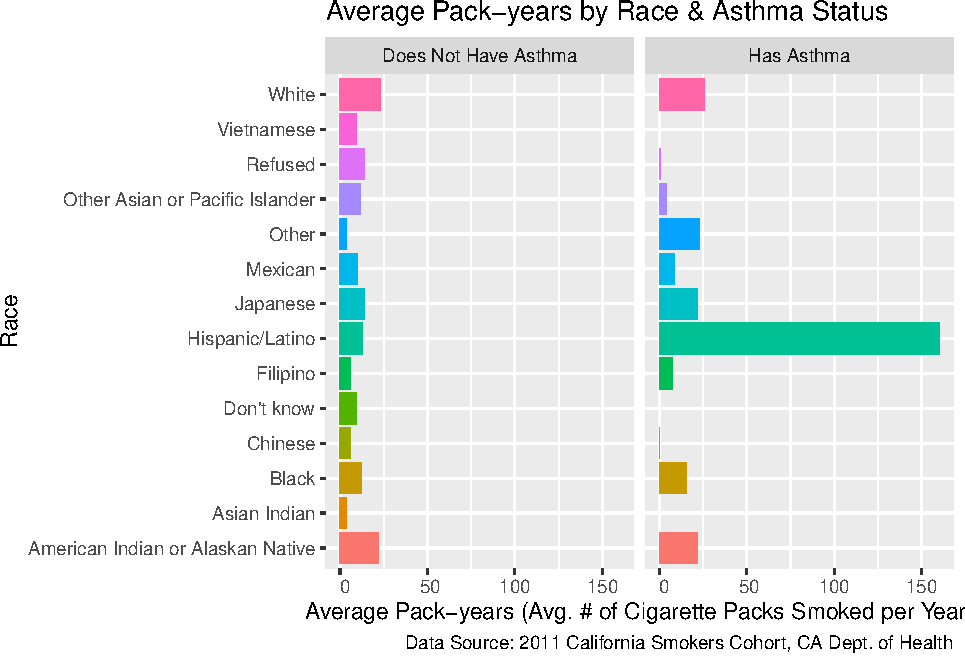
\includegraphics{Milestone_4_files/figure-latex/bar graph of cigarette pack-years by race and asthma-1.pdf}
\newpage

\begin{Shaded}
\begin{Highlighting}[]
\NormalTok{avg\_pack\_years\_race\_heartdis }\SpecialCharTok{\%\textgreater{}\%}
  \FunctionTok{drop\_na}\NormalTok{(}\FunctionTok{c}\NormalTok{(heartdis, avg\_pack\_years)) }\SpecialCharTok{\%\textgreater{}\%}
  \FunctionTok{ggplot}\NormalTok{(}\FunctionTok{aes}\NormalTok{(}\AttributeTok{x =}\NormalTok{ race, }\AttributeTok{y =}\NormalTok{ avg\_pack\_years)) }\SpecialCharTok{+}
  \FunctionTok{geom\_bar}\NormalTok{(}\FunctionTok{aes}\NormalTok{(}\AttributeTok{fill=}\NormalTok{race), }\AttributeTok{stat=}\StringTok{"identity"}\NormalTok{, }\AttributeTok{position =} \StringTok{"dodge"}\NormalTok{) }\SpecialCharTok{+}
  \FunctionTok{coord\_flip}\NormalTok{() }\SpecialCharTok{+}
  \FunctionTok{guides}\NormalTok{(}\AttributeTok{fill =} \StringTok{"none"}\NormalTok{) }\SpecialCharTok{+}
  \FunctionTok{labs}\NormalTok{(}\AttributeTok{x =} \StringTok{"Race"}\NormalTok{,}
       \AttributeTok{y =} \StringTok{"Average Pack{-}years (Avg. \# of Cigarette Packs Smoked per Year)"}\NormalTok{,}
  \AttributeTok{title =} \StringTok{"Average Pack{-}years by Race \& Heart Disease Status"}\NormalTok{,}
  \AttributeTok{caption =} \StringTok{"Data Source: 2011 California Smokers Cohort, CA Dept. of Health"}\NormalTok{) }\SpecialCharTok{+}
  \FunctionTok{scale\_y\_continuous}\NormalTok{(}\AttributeTok{labels =} \ControlFlowTok{function}\NormalTok{(x) }\FunctionTok{format}\NormalTok{(x,}\AttributeTok{big.mark=}\StringTok{","}\NormalTok{,}
                                                     \AttributeTok{scientific=}\ConstantTok{FALSE}\NormalTok{)) }\SpecialCharTok{+}
  \FunctionTok{facet\_wrap}\NormalTok{(}\SpecialCharTok{\textasciitilde{}}\NormalTok{ heartdis, }\AttributeTok{labeller =} \FunctionTok{labeller}\NormalTok{(}\AttributeTok{heartdis =}
                                      \FunctionTok{c}\NormalTok{(}\StringTok{"No"} \OtherTok{=} \StringTok{"Does Not Have Heart Disease"}\NormalTok{,}
                                        \StringTok{"Yes"} \OtherTok{=} \StringTok{"Has Heart Disease"}\NormalTok{)))}
\end{Highlighting}
\end{Shaded}

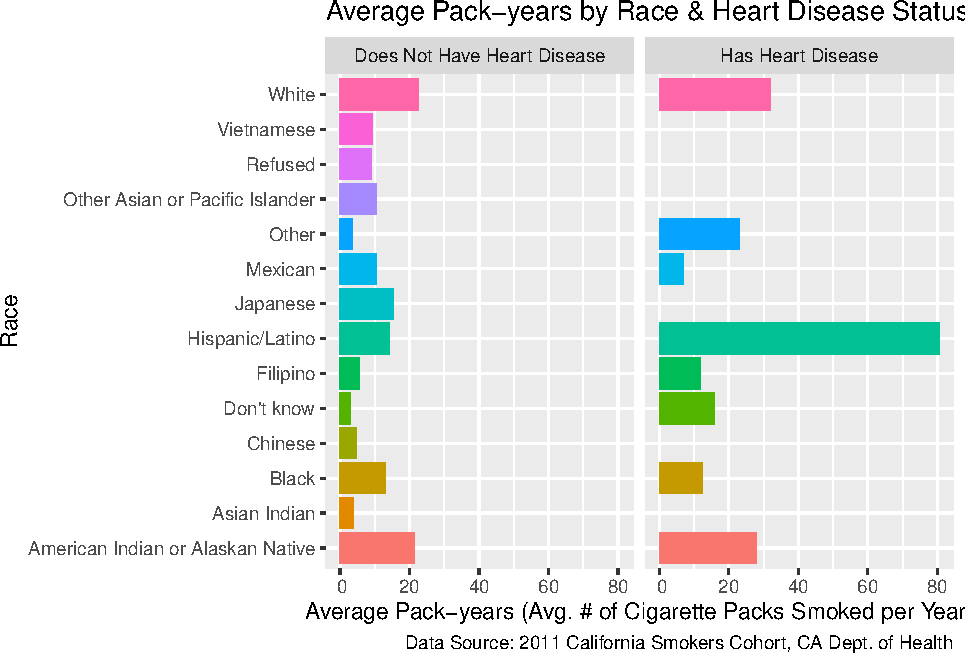
\includegraphics{Milestone_4_files/figure-latex/bar graph of cigarette pack-years by race and heartdis-1.pdf}
\newpage

\begin{Shaded}
\begin{Highlighting}[]
\NormalTok{avg\_pack\_years\_race\_diabetes }\SpecialCharTok{\%\textgreater{}\%}
  \FunctionTok{drop\_na}\NormalTok{(}\FunctionTok{c}\NormalTok{(diabetes, avg\_pack\_years)) }\SpecialCharTok{\%\textgreater{}\%}
  \FunctionTok{ggplot}\NormalTok{(}\FunctionTok{aes}\NormalTok{(}\AttributeTok{x =}\NormalTok{ race, }\AttributeTok{y =}\NormalTok{ avg\_pack\_years)) }\SpecialCharTok{+}
  \FunctionTok{geom\_bar}\NormalTok{(}\FunctionTok{aes}\NormalTok{(}\AttributeTok{fill=}\NormalTok{race), }\AttributeTok{stat=}\StringTok{"identity"}\NormalTok{, }\AttributeTok{position =} \StringTok{"dodge"}\NormalTok{) }\SpecialCharTok{+}
  \FunctionTok{coord\_flip}\NormalTok{() }\SpecialCharTok{+}
  \FunctionTok{guides}\NormalTok{(}\AttributeTok{fill =} \StringTok{"none"}\NormalTok{) }\SpecialCharTok{+}
  \FunctionTok{labs}\NormalTok{(}\AttributeTok{x =} \StringTok{"Race"}\NormalTok{,}
       \AttributeTok{y =} \StringTok{"Average Pack{-}years (Avg. \# of Cigarette Packs Smoked per Year)"}\NormalTok{,}
  \AttributeTok{title =} \StringTok{"Average Pack{-}years by Race \& Diabetes Status"}\NormalTok{,}
  \AttributeTok{caption =} \StringTok{"Data Source: 2011 California Smokers Cohort, CA Dept. of Health"}\NormalTok{) }\SpecialCharTok{+}
  \FunctionTok{scale\_y\_continuous}\NormalTok{(}\AttributeTok{labels =} \ControlFlowTok{function}\NormalTok{(x) }\FunctionTok{format}\NormalTok{(x,}\AttributeTok{big.mark=}\StringTok{","}\NormalTok{,}
                                                     \AttributeTok{scientific=}\ConstantTok{FALSE}\NormalTok{)) }\SpecialCharTok{+}
  \FunctionTok{facet\_wrap}\NormalTok{(}\SpecialCharTok{\textasciitilde{}}\NormalTok{ diabetes,}
             \AttributeTok{labeller =} \FunctionTok{labeller}\NormalTok{(}\AttributeTok{diabetes =} \FunctionTok{c}\NormalTok{(}\StringTok{"No"} \OtherTok{=} \StringTok{"Does Not Have Diabetes"}\NormalTok{,}
                                                      \StringTok{"Yes"} \OtherTok{=} \StringTok{"Has Diabetes"}\NormalTok{)))}
\end{Highlighting}
\end{Shaded}

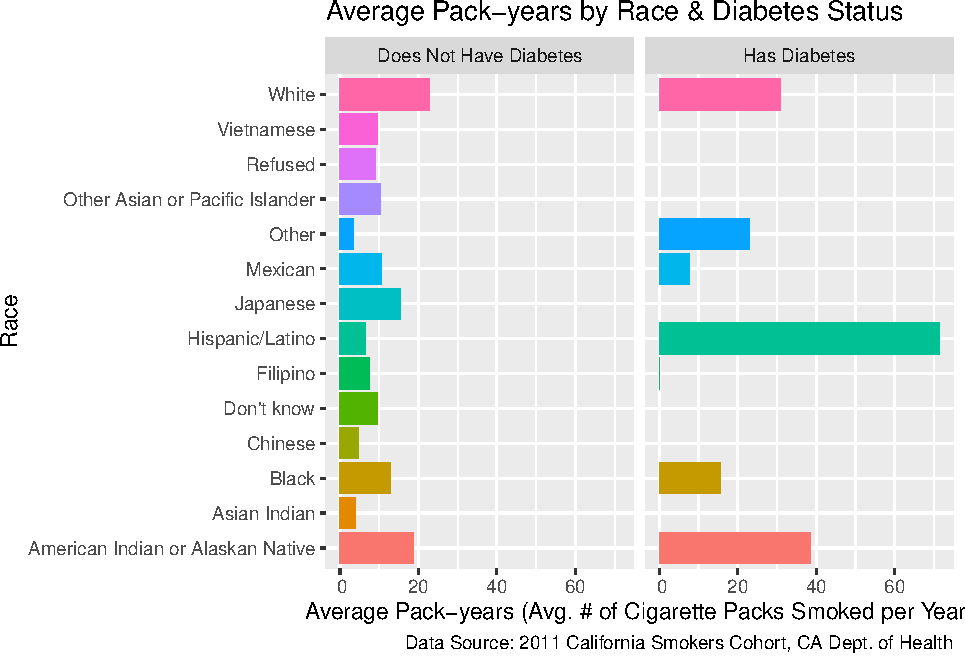
\includegraphics{Milestone_4_files/figure-latex/bar graph of cigarette pack-years by race and diabetes-1.pdf}
\newpage

\begin{Shaded}
\begin{Highlighting}[]
\NormalTok{avg\_pack\_years\_race\_othmenill }\SpecialCharTok{\%\textgreater{}\%}
  \FunctionTok{drop\_na}\NormalTok{(}\FunctionTok{c}\NormalTok{(othmenill, avg\_pack\_years)) }\SpecialCharTok{\%\textgreater{}\%}
  \FunctionTok{ggplot}\NormalTok{(}\FunctionTok{aes}\NormalTok{(}\AttributeTok{x =}\NormalTok{ race, }\AttributeTok{y =}\NormalTok{ avg\_pack\_years)) }\SpecialCharTok{+}
  \FunctionTok{geom\_bar}\NormalTok{(}\FunctionTok{aes}\NormalTok{(}\AttributeTok{fill=}\NormalTok{race), }\AttributeTok{stat=}\StringTok{"identity"}\NormalTok{, }\AttributeTok{position =} \StringTok{"dodge"}\NormalTok{) }\SpecialCharTok{+}
  \FunctionTok{coord\_flip}\NormalTok{() }\SpecialCharTok{+}
  \FunctionTok{guides}\NormalTok{(}\AttributeTok{fill =} \StringTok{"none"}\NormalTok{) }\SpecialCharTok{+}
  \FunctionTok{labs}\NormalTok{(}\AttributeTok{x =} \StringTok{"Race"}\NormalTok{,}
       \AttributeTok{y =} \StringTok{"Average Pack{-}years (Avg. \# of Cigarette Packs Smoked per Year)"}\NormalTok{,}
  \AttributeTok{title =} \StringTok{"Average Pack{-}years by Race \& Mental Illness Status"}\NormalTok{,}
  \AttributeTok{caption =} \StringTok{"Data Source: 2011 California Smokers Cohort, CA Dept. of Health"}\NormalTok{) }\SpecialCharTok{+}
  \FunctionTok{scale\_y\_continuous}\NormalTok{(}\AttributeTok{labels =} \ControlFlowTok{function}\NormalTok{(x) }\FunctionTok{format}\NormalTok{(x,}\AttributeTok{big.mark=}\StringTok{","}\NormalTok{,}
                                                     \AttributeTok{scientific=}\ConstantTok{FALSE}\NormalTok{)) }\SpecialCharTok{+}
  \FunctionTok{facet\_wrap}\NormalTok{(}\SpecialCharTok{\textasciitilde{}}\NormalTok{ othmenill, }\AttributeTok{labeller =} \FunctionTok{labeller}\NormalTok{(}\AttributeTok{othmenill =}
                                      \FunctionTok{c}\NormalTok{(}\StringTok{"No"} \OtherTok{=} \StringTok{"Does Not Have Mental Illness"}\NormalTok{,}
                                        \StringTok{"Yes"} \OtherTok{=} \StringTok{"Has Mental Illness"}\NormalTok{)))}
\end{Highlighting}
\end{Shaded}

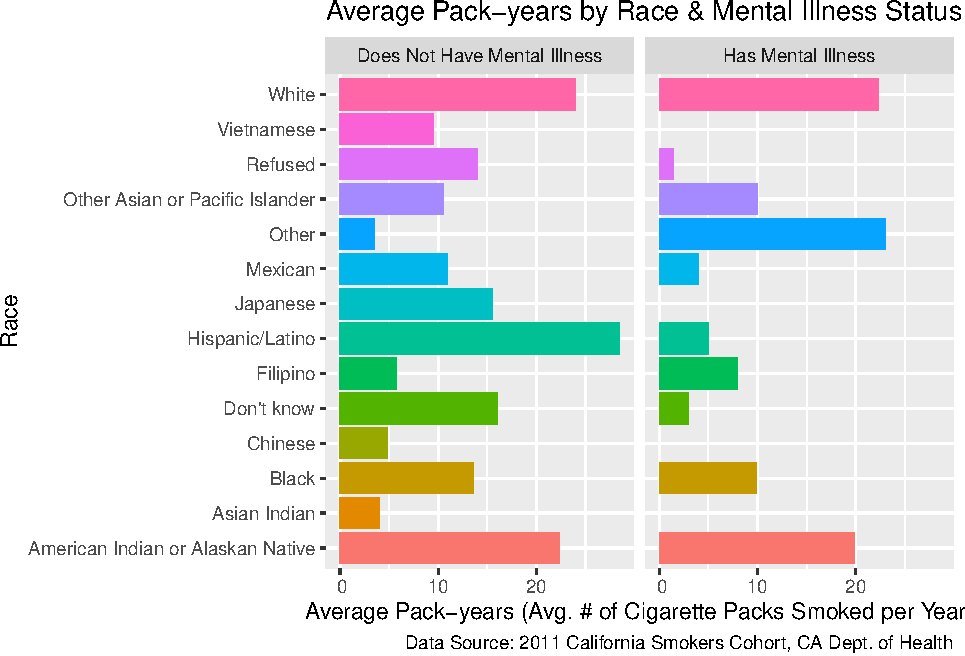
\includegraphics{Milestone_4_files/figure-latex/bar graph of cigarette pack-years by race and othmenill-1.pdf}
\newpage

\emph{\textbf{Interpretation of the Four Graphs of Average Pack-years by
Race and Disease:}} \newline Except for mental illness, among
individuals who reported that they do not have asthma, heart disease,
and/or diabetes, those who identified as either ``White'' or ``American
Indian or Alaskan Native'' by race appear to have a greater number of
average pack-years (i.e., average number of cigarette packs smoked per
year) compared to other races in the 2011 California Smokers Cohort.

Except for mental illness, among individuals who reported that they do
have asthma, heart disease, and/or diabetes, those who identified as
``Hispanic/Latino'' by race appear to have the greatest number of
average pack-years (i.e., average number of cigarette packs smoked per
year) compared to other races in the 2011 California Smokers Cohort.

\newpage

\hypertarget{work-in-progress}{%
\subsection{Work in progress:}\label{work-in-progress}}

\#\#OUR GROUP'S RESEARCH QUESTION (For reference only to help us think
of relevant \#graphs - delete later): ``For this project, we aim to
investigate how tobacco use primarily impacts mental illness among
smokers in California in 2011, as well as explore how race and location
of cigarette purchase can impact disease status.''

Visualizations (3 total) \textbf{one print quality tables per scenario}
With Kable: pack-years vs.~asthma/heart disease/diabetes/mental illness
(1 table)

``Compare the average number of pack-years by at least four disease
outcomes (e.g.~asthma, heart disease, diabetes, physical illness, and/or
mental illness). Provide a print-quality table that shows the average
number of pack-years and the disease outcomes.''

Average number of pack-years = pack\_years/sum(pack\_years)

\textbf{one print quality plot or chart per scenario} With ggplot: 1 bar
graph (x = disease, y = pack-years) \textbf{one additional table or
plot} With ggplot: dodged bar chart with (x = cigarette purchase
location, aes(fill = othmenill) to view cigarette purchase location and
mental illness status

\hypertarget{each-visual-should-include}{%
\section{Each visual should include:}\label{each-visual-should-include}}

\textbf{code} \textbf{legend (if necessary) } Unless we decide to input
a third variable in a graph.

\textbf{interpretation (1 to 2 sentences)}

\#\#PDF should be prepared for presentation \textbf{each part of
milestone on new page} \textbf{only necessary info outputted}
\textbf{show work with ``echo''}

\end{document}
